\documentclass[11pt,a4paper,final,addpoints]{exam}
\usepackage[utf8]{inputenc}
\usepackage[portuguese]{babel}
\usepackage[T1]{fontenc}
\usepackage{amsmath}
\usepackage{amsfonts}
\usepackage{amssymb}
\usepackage{graphicx}
\usepackage{pstricks,pst-circ,pst-osci}
\usepackage[left=1cm,right=1cm,top=2cm,bottom=2cm,twoside]{geometry}
\author{Tiago Á. Oliveira}
\title{Relatorio Individual}


\pagestyle{headandfoot}

\extraheadheight[1.5in]{-.25in}

\firstpageheader{\textbf{Turma P13}}
{
\includegraphics[scale=1]{figs/logo_UA}
\linebreak\linebreak
\LARGE\textbf{Eletricidade \& Magnetismo}
\normalsize\linebreak
(2014-2015)
\linebreak\linebreak
\textbf{Relat\'{o}rio Individual de Laborat\'{o}rio}
\linebreak
12 de dezembro de 2014
\linebreak}
%{\textbf{Vers\~{a}o A}}
{\textbf{Vers\~{a}o B}}

\runningheader{\oddeven{}{Eletricidade \& Magnetismo (2014-15)}}{}{\oddeven{Relat\'{o}rio Individual de Laborat\'{o}rio}{}}
\headrule

\footrule
\footer{\oddeven{}{P\'{a}gina \thepage}}{\iflastpage{Fim!}}{\oddeven{P\'{a}gina \thepage}{}}

% RESPOSTAS 
\printanswers
\renewcommand{\solutiontitle}{\noindent\textbf{Resposta:}}


\begin{document}
\begin{center}
\makebox[\textwidth]{\textbf{Nome:}~\underline{\hspace{11cm}}~\textbf{N.\textsuperscript{o} Mecanogr\'{a}fico:}~\underline{\hspace{2.5cm}}}
\end{center}

\noindent\textbf{Recomenda\c{c}\~{o}es:}
\begin{itemize}
\item O relat\'{o}rio \'{e} realizado individualmente;

\item Leia atentamente todo o enunciado da prova e se tiver d\'{u}vidas coloque-as ao docente;

\item Tem a dura\c{c}\~{a}o exata de 2 horas, sem qualquer toler\^{a}ncia;

\item O enunciado do relat\'{o}rio tem 2 vers\~{o}es distintas mas de igual dificuldade. 

\underline{Dever\~{a}o indicar a vers\~{a}o (A ou B) no in\'{i}cio da folha de resposta};

\item \underline{Dever\~{a}o justificar todas as respostas};

\item N\~{a}o ser\'{a} permitida a consulta dos guias, fichas ou dos registos efetuados durante as aulas;

\item N\~{a}o haver\'{a} formul\'{a}rio para as leis fundamentais (Lei de Ohm, Kirschoff, Faraday, Lenz, etc.). Equa\c{c}\~{o}es de dedu\c{c}\~{a}o complexa/demorada, caso sejam necess\'{a}rias, estar\~{a}o presentes no enunciado;

\item Podem usar m\' {a}quina de calcular com capacidades gr\'{a}ficas;

\item O uso do computador/tablet est\'{a} restringido apenas para uso no tratamento de dados (Excel, MatLAB, etc.) n\~{a}o podendo ser usado para consulta de PDF's ou liga\c{c}\~{a}o \`{a} Internet;

\item O telem\'{o}vel dever\'{a} estar desligado durante a prova.
\end{itemize}

\noindent\textbf{Cota\c{c}\~{o}es:}
\begin{center}
\hqword{\textit{Quest\~{a}o}}
\hpword{\textit{Pontos}}
\hsword{\textit{Obtidos}}
\htword{\textbf{Total}}
\gradetable[h][questions]
\linebreak
\end{center}

\noindent\textbf{Constantes fundamentais:}
\begin{center}
\begin{tabular}{cc}
$\varepsilon_0 = 8.85\times10^{-12}~\text{C}^2/\text{Nm}^2$ & $\mu_0 = 4\pi\times10^{-7}~\text{N}/\text{A}^2$ \\ 
$e=1.60\times10^{-19}~\text{C}$ & $m_e=9.11\times10^{-31}~\text{kg}$ \\ 
\end{tabular} 
\end{center}


\boxedpoints
\pointsinmargin
\newpage
\begin{questions}
% Versao P13 - A
%%
%

\question
\textbf{Trabalho Pr\'{a}tico 1 : Eletrost\'{a}tica}

Recorde o Trabalho Pr\'{a}tico 1, no qual determinou a capacidade el\'{e}trica de uma esfera condutora.

Neste trabalho aplicou diversos potenciais elevados a uma esfera condutora de raio $R\pm\Delta R=4.50\pm0.05~\text{cm}$, adquirindo esta uma carga. Os valores dessa carga $Q$, para diferentes potenciais aplicados $V$, est\~{a}o registados na Tabela~\ref{tab:qesfera}.

\begin{table}[h]
\centering
\caption{\label{tab:qesfera}Carga ($Q$) da esfera em fun\c{c}\~{a}o do potencial ($V$) aplicado.}
\begin{tabular}{|c|c|c|c|c|c|c|}
\hline 
$V\pm 0.01$ (kV) & 0.52 & 1.85 & 3.14 & 3.93 & 5.39 & 6.43 \\ 
\hline 
$Q\pm 1$ (nC) & 12 & 17 & 25 & 29 & 35 & 41 \\ 
\hline 
\end{tabular} 
\end{table}

\begin{parts}
\part[15]
A carga da esfera n\~{a}o \'{e} medida diretamente. Explique sucintamente, como se determina o valor da carga.

\part[25]
Determine o valor experimental da capacidade el\'{e}trica da esfera $C_\text{esfera}$ e respectivo erro. (Nota: N\~{a}o precisa de representar graficamente os valores experimentais bem como a reta da lineariza\c{c}\~{a}o.)

\part[10]
Compare o valor experimental com o valor esperado, sabendo que a tens\~{a}o aplicada \`{a} esfera condutora \'{e} proporcional \`{a} carga $Q$ de acordo com a Eq.~\ref{eq:vpropq}. Comente o resultado.

\begin{equation}
\label{eq:vpropq}
V=\frac{1}{4\pi\varepsilon_0 R}Q
\end{equation}
\end{parts}
%\question
\textbf{Trabalho Pr\'{a}tico 6 : Indu\c{c}\~{a}o Eletromagn\'{e}tica}

Recorde o trabalho pr\'{a}tico sobre a Indu\c{c}\~{a}o eletromagn\'{e}tica.

\begin{parts}
\part[10]
Na primeira parte deste trabalho montou o circuito da Fig.~\ref{fig:bobinas}, com o objetivo de estudar a Lei de Faraday e de Lenz.

Descreva o que observou no movimento dos ponteiros do galvan\'{o}metro, quando ligou a fonte de tens\~{a}o e, \`{a} luz das leis de Faraday e de Lenz, indique o sentido da corrente induzida no circuito da bobina 2.

\begin{figure}[h]
\centering
\begin{pspicture}[showgrid=false](9,5)
\pnodes(1,1){A}(1,4){B}(4,4){C}(4,1){D}(5,1){E}(5,4){F}(8,4){G}(8,1){H}
\vdc[labeloffset=1](A)(D){$15~\text{V}$}
\resistor[dipolestyle=zigzag,labelangle=:U](A)(B){$5~\Omega$}
\coil[dipolestyle=curved,
      labelangle=:U,
      intensitylabel=$I$,
      labeloffset=-.5](C)(D){$1200~\text{esp.}$}
\newSwitch[tensionlabel=Bobina 1,
           tensioncolor=white,
           tensionlabeloffset=0.7](B)(C){}

\coil[dipolestyle=curved,
      labelangle=:U,
      labeloffset=-.5](E)(F){$3600~\text{esp.}$}
\wire(G)(H)      
\circledipole[tensionlabel=Bobina 2,
           tensioncolor=white,
           tensionlabeloffset=0.7,
           labeloffset=0.0](F)(G){\Large\textbf{G}}
\wire(E)(H)

\end{pspicture}
\caption{\label{fig:bobinas}}
\end{figure}

\part\label{part:m}
Considere um circuito no qual est\~{a}o ligados em s\'{e}rie um gerador de sinal, uma resist\^{e}ncia de $R\pm\Delta R=100\pm5~\Omega$ e um solenoide (daqui em diante referido como \emph{prim\'{a}rio}) de raio $r\pm\Delta r=1.38\pm0.01~\text{cm}$ e $N/l\pm\Delta N/l=3000\pm15$ espiras por metro. Uma bobina (daqui em diante referida como \emph{secund\'{a}rio}) de $N_b\pm\Delta N_b=1200\pm6$ espiras envolve o \emph{prim\'{a}rio}. Aplica-se um sinal triangular ao circuito \emph{prim\'{a}rio} tendo-se observado nos terminais da resist\^{e}ncia o sinal do Canal A da Fig.~\ref{fig:osci} (\emph{tracejado}). O sinal induzido no \emph{secund\'{a}rio} \'{e} o que se observa no Canal B da mesma figura (\emph{cheio}).

\begin{subparts}
\subpart[30]
Determine o coeficiente de indu\c{c}\~{a}o m\'{u}tua observado e compare-o com o esperado, sabendo que a for\c{c}a eletromotriz (f.e.m.) induzida no \emph{secund\'{a}rio} \'{e} dada pela Eq.~\ref{eq:fem}.

\begin{equation}
\label{eq:fem}
\varepsilon=\pi\mu_0\frac{N}{l}r^2N_b\frac{\mathrm d i}{\mathrm d t}
\end{equation}

\begin{figure}[h]
\begin{center}
\newpsstyle{Dash}{linestyle=dashed,
linecolor=black,linewidth=0.035,plotpoints=50}
\psscalebox{1}{
\Oscillo[Wave1=\TriangleA,
         Wave2=\RectangleB,
    amplitude1=4.00,
    amplitude2=-0.3,
       period1=1.2,
       period2=1.2,
        phase1=0.0,
        phase2=0.0,        
    sensivity1=1.0,
    sensivity2=0.2,
       timediv=0.15,
       offset2=-0.9,        
    plotstyle1=Dash,
      AllColor=false]}
\caption{\label{fig:osci}Visor do oscilosc\'{o}pio. O Canal A est\'{a} representado a tracejado enquanto o Canal B a cheio.}
\end{center}
\end{figure}

\subpart[15]
Justique convenientemente a forma do sinal induzido (Fig.~\ref{fig:osci}~-~\textit{cheio})

\subpart[10]
Explique como efetuou as liga\c{c}\~{o}es \`{a} terra dos canais do oscil\'{o}scopio e do gerador de sinais. Justifique convenientemente a resposta.

\subpart[10]
Se o sinal aplicado (Canal A) fosse quadrangular, o sinal induzido (Canal B) seria triangular?

\end{subparts}
\end{parts}
%\newpage
%\question
\textbf{Trabalho Pr\'{a}tico 5 : Bobinas de Helmholtz}

Recorde o trabalho pr\'{a}tico sobre o estudo do campo magn\'{e}tico produzido pelas Bobinas de Helmholtz. Os resultados experimentais obtidos est\~{a}o representados no gr\'{a}fico da Fig.~\ref{fig:helmholtz}. Cada bobina tem de raio $R=3.5~\text{cm}$.

\begin{figure}[ht]
\centering
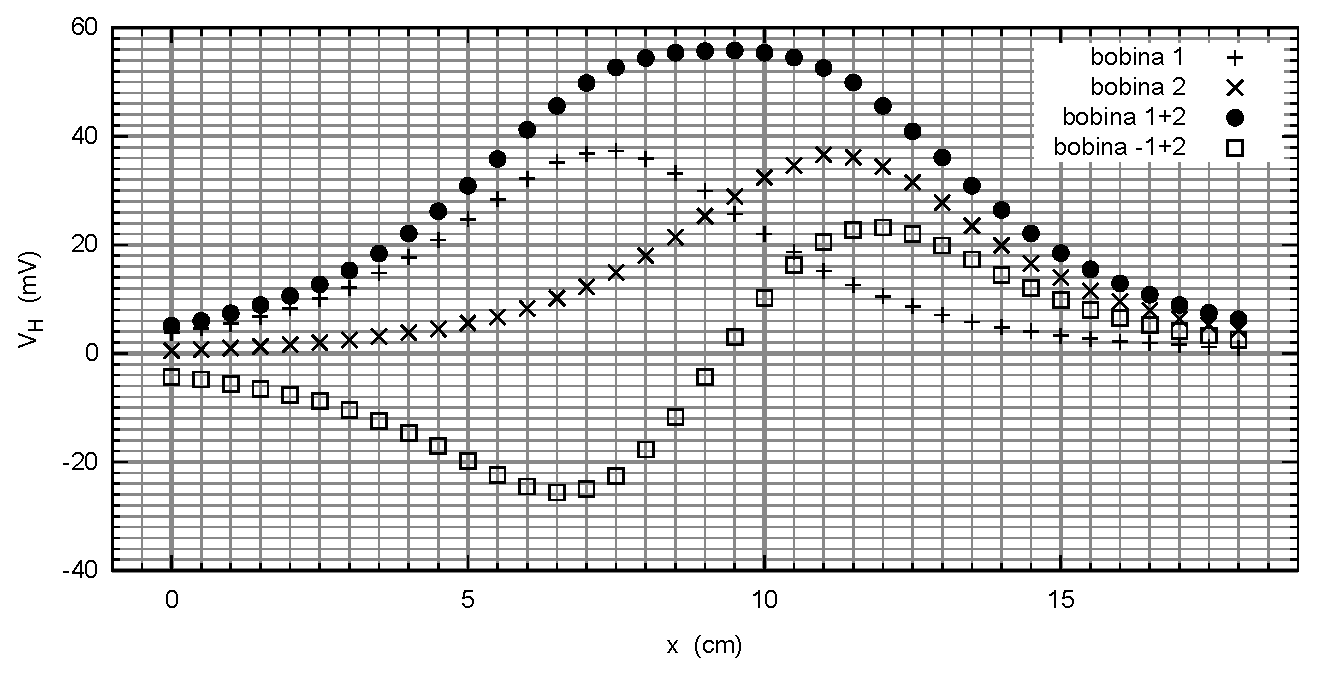
\includegraphics[scale=0.8]{gnuplot/helmholtz.eps}
\caption{\label{fig:helmholtz}Tens\~{a}o de Hall ao longo do eixo das bobinas.}
\end{figure}

\begin{parts}
\part[20]
A medi\c{c}\~{a}o do campo foi feita com recurso a uma sonda de efeito de Hall. Para a calibra\c{c}\~{a}o desta usou um solenoide padr\~{a}o. Diga em que posi\c{c}\~{a}o do solenoide colocou a sonda e porqu\^{e}.

\part[15]
Sabendo que a constante de calibra\c{c}\~{a}o da sonda $C_c \pm \Delta Cc = 34.9 \pm 0.5~\text{(mT/V)}$, determine o valor do campo magn\'{e}tico para a Bobina 2 e respetivo erro, na posi\c{c}\~{a}o $x=11.5~\text{cm}$.

\part[10]
Indique, justificando, se trabalhou em configura\c{c}\~{a}o de Helmholtz e indique tamb\'{e}m a principal vantagem desta configura\c{c}\~{a}o de bobinas.

\part[15]
Conclua, atrav\'{e}s do gr\'{a}fico, se se verifica ou n\~{a}o o princ\'{i}pio da sobreposi\c{c}\~{a}o do campo magnetico no caso em que as bobinas t\^{e}m corrente a fluir em sentidos opostos.

\part[15]
Determine o n\'{u}mero de espiras da bobina 2 se nesta estiver a fluir uma corrente de $I=0.585~\text{A}$, sabendo que o campo magn\'{e}tico por uma espira ao longo do seu eixo \'{e} dado pela Eq.~\ref{eq:coilfield}.

\begin{equation}
\label{eq:coilfield}
B\left(x\right)=\frac{\mu_0}{2}\frac{IR^2}{\left(R^2+x^2\right)^{3/2}}
\end{equation}
\end{parts}

% Versao P13 - B
%
%

\question
\textbf{Trabalho Pr\'{a}tico 1 : Eletrost\'{a}tica}

Recorde o Trabalho Pr\'{a}tico 1, no qual determinou a capacidade el\'{e}trica de uma esfera condutora.

Neste trabalho aplicou diversos potenciais elevados a uma esfera condutora de raio $R\pm\Delta R=4.50\pm0.05~\text{cm}$, adquirindo esta uma carga. Os valores dessa carga $Q$, para diferentes potenciais aplicados $V$, est\~{a}o registados na Tabela~\ref{tab:qesfera}.

\begin{table}[h]
\centering
\caption{\label{tab:qesfera}Carga ($Q$) da esfera em fun\c{c}\~{a}o do potencial ($V$) aplicado.}
\begin{tabular}{|c|c|c|c|c|c|c|}
\hline 
$V\pm 0.01$ (kV) & 0.52 & 1.85 & 3.14 & 3.93 & 5.39 & 6.43 \\ 
\hline 
$Q\pm 1$ (nC) & 12 & 17 & 25 & 29 & 35 & 41 \\ 
\hline 
\end{tabular} 
\end{table}

\begin{parts}
\part[15]
A carga da esfera \'{e} medida indiretamente usando um electr\'{o}metro. Explique sucintamente, como este funciona e porque se deve manter o copo do electr\'{o}metro ligado \`{a} terra entre cada medi\c{c}\~{a}o.

\part[25]
Determine o valor experimental da capacidade el\'{e}trica da esfera $C_\text{esfera}$ e respectivo erro. (Nota: N\~{a}o precisa de representar graficamente os valores experimentais bem como a reta da lineariza\c{c}\~{a}o.)

\part[10]
Compare o valor experimental com o valor esperado, sabendo que a carga $Q$ adquirida pela esfera condutora \'{e} proporcional \`{a} tens\~{a}o aplicada \`{a} esfera de acordo com a Eq.~\ref{eq:vpropq}. Comente o resultado.

\begin{equation}
\label{eq:vpropq}
Q=4\pi\varepsilon_0 R V
\end{equation}
\end{parts}
\question
\textbf{Trabalho Pr\'{a}tico 6 : Indu\c{c}\~{a}o Eletromagn\'{e}tica}

Recorde o trabalho pr\'{a}tico sobre a Indu\c{c}\~{a}o eletromagn\'{e}tica.

\begin{parts}
\part[10]
Na primeira parte deste trabalho montou o circuito da Fig.~\ref{fig:bobinas}, com o objetivo de estudar a Lei de Faraday e de Lenz.

Descreva o que observou no movimento dos ponteiros do galvan\'{o}metro quando, ap\'{o}s ter mantido o circuito ligado, desligou a fonte de tens\~{a}o e, \`{a} luz das leis de Faraday e de Lenz, indique o sentido da corrente induzida nesse instante (em que desligou) no circuito da bobina 2.

\begin{figure}[h]
\centering
\begin{pspicture}[showgrid=false](9,5)
\pnodes(1,1){A}(1,4){B}(4,4){C}(4,1){D}(5,1){E}(5,4){F}(8,4){G}(8,1){H}
\vdc[labeloffset=1](A)(D){$15~\text{V}$}
\resistor[dipolestyle=zigzag,labelangle=:U](A)(B){$5~\Omega$}
\coil[dipolestyle=curved,
      labelangle=:U,
      intensitylabel=$I$,
      labeloffset=-.5](C)(D){$1200~\text{esp.}$}
\newSwitch[tensionlabel=Bobina 1,
           tensioncolor=white,
           ison=false,
           tensionlabeloffset=0.7](B)(C){}

\coil[dipolestyle=curved,
      labelangle=:U,
      labeloffset=-.5](E)(F){$3600~\text{esp.}$}
\wire(G)(H)      
\circledipole[tensionlabel=Bobina 2,
           tensioncolor=white,
           tensionlabeloffset=0.7,
           labeloffset=0.0](F)(G){\Large\textbf{G}}
\wire(E)(H)

\end{pspicture}
\caption{\label{fig:bobinas}}
\end{figure}

\part\label{part:m}
Considere um circuito no qual est\~{a}o ligados em s\'{e}rie um gerador de sinal, uma resist\^{e}ncia de $R\pm\Delta R=100\pm5~\Omega$ e um solenoide (daqui em diante referido como \emph{prim\'{a}rio}) de raio $r\pm\Delta r=1.38\pm0.01~\text{cm}$ e $N/l\pm\Delta N/l=3000\pm15$ espiras por metro. Uma bobina (daqui em diante referida como \emph{secund\'{a}rio}) de $N_b\pm\Delta N_b=1200\pm6$ espiras envolve o \emph{prim\'{a}rio}. Aplica-se um sinal triangular ao circuito \emph{prim\'{a}rio} tendo-se observado nos terminais da resist\^{e}ncia o sinal do Canal A da Fig.~\ref{fig:osci} (\emph{tracejado}). O sinal induzido no \emph{secund\'{a}rio} \'{e} o que se observa no Canal B da mesma figura (\emph{cheio}).

\begin{subparts}
\subpart[30]
Determine o coeficiente de indu\c{c}\~{a}o m\'{u}tua observado e compare-o com o esperado, sabendo que a for\c{c}a eletromotriz (f.e.m.) induzida no \emph{secund\'{a}rio} \'{e} dada pela Eq.~\ref{eq:fem}.

\begin{equation}
\label{eq:fem}
\varepsilon=\pi\mu_0\frac{N}{l}r^2N_b\frac{\mathrm d i}{\mathrm d t}
\end{equation}

\begin{figure}[h]
\begin{center}
\newpsstyle{Dash}{linestyle=dashed,
linecolor=black,linewidth=0.035,plotpoints=50}
\psscalebox{1}{
\Oscillo[Wave1=\TriangleA,
         Wave2=\RectangleB,
    amplitude1=4.00,
    amplitude2=-0.3,
       period1=1.2,
       period2=1.2,
        phase1=0.0,
        phase2=0.0,        
    sensivity1=1.0,
    sensivity2=0.2,
       timediv=0.15,
       offset2=+0.9,        
    plotstyle1=Dash,
      AllColor=false]}
\caption{\label{fig:osci}Visor do oscilosc\'{o}pio. O Canal A est\'{a} representado a tracejado enquanto o Canal B a cheio.}
\end{center}
\end{figure}

\subpart[15]
Justique convenientemente a forma do sinal induzido (Fig.~\ref{fig:osci}~-~\textit{cheio}).

\subpart[10]
Porque \'{e} que o sinal induzido (Fig.~\ref{fig:osci}~-~\textit{cheio}) apresenta flutua\c{c}\~{o}es nas extremidades?

\subpart[10]
Se o sinal aplicado (Canal A) fosse do tipo "dente-de-serra", o sinal induzido (Canal B) seria triangular?

\end{subparts}
\end{parts}
\newpage
\question
\textbf{Trabalho Pr\'{a}tico 5 : Bobinas de Helmholtz}

Recorde o trabalho pr\'{a}tico sobre o estudo do campo magn\'{e}tico produzido pelas Bobinas de Helmholtz. Os resultados experimentais obtidos est\~{a}o representados no gr\'{a}fico da Fig.~\ref{fig:helmholtz}. Cada bobina tem de raio $R=3.5~\text{cm}$.

\begin{figure}[ht]
\centering
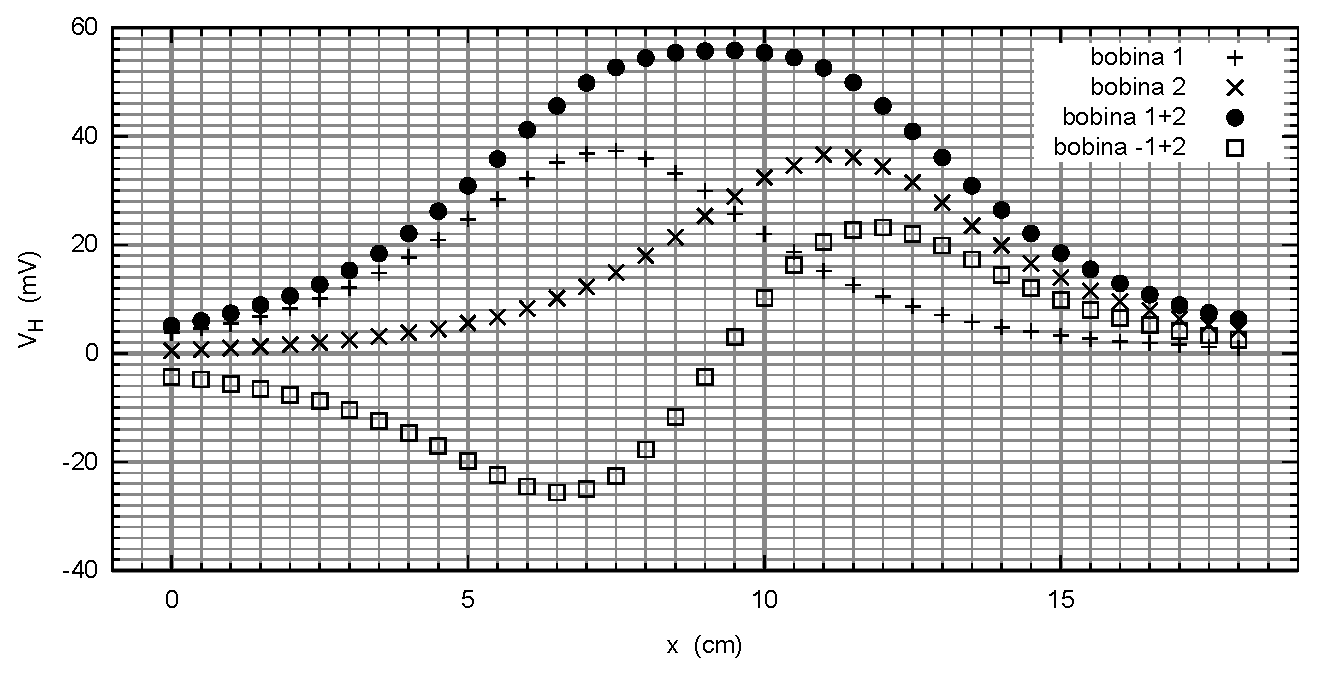
\includegraphics[scale=0.8]{gnuplot/helmholtz.eps}
\caption{\label{fig:helmholtz}Tens\~{a}o de Hall ao longo do eixo das bobinas.}
\end{figure}

\begin{parts}
\part[20]
A medi\c{c}\~{a}o do campo foi feita com recurso a uma sonda de efeito de Hall. Explique o que \'{e} o efeito de Hall num semicondutor cujos portadores de carga maiorit\'{a}rios s\~{a}o positivos. (Nota: Pode recorrer a esbo\c{c}o gr\'{a}fico para ilustrar a sua resposta.)

\part[15]
Sabendo que a constante de calibra\c{c}\~{a}o da sonda $C_c \pm \Delta Cc = 34.9 \pm 0.5~\text{(mT/V)}$, determine o valor do campo magn\'{e}tico para a Bobina 1 e respetivo erro, na posi\c{c}\~{a}o $x=7.5~\text{cm}$.

\part[10]
Indique, justificando, se trabalhou em configura\c{c}\~{a}o de Helmholtz e indique tamb\'{e}m a principal vantagem desta configura\c{c}\~{a}o de bobinas.

\part[15]
Conclua, atrav\'{e}s do gr\'{a}fico, se se verifica ou n\~{a}o o princ\'{i}pio da sobreposi\c{c}\~{a}o do campo magnetico no caso em que as bobinas t\^{e}m corrente a fluir no mesmo sentido.

\part[15]
Determine o n\'{u}mero de espiras da bobina 1 se nesta estiver a fluir uma corrente de $I=0.585~\text{A}$, sabendo que o campo magn\'{e}tico por uma espira ao longo do seu eixo \'{e} dado pela Eq.~\ref{eq:coilfield}.

\begin{equation}
\label{eq:coilfield}
B\left(x\right)=\frac{\mu_0}{2}\frac{IR^2}{\left(R^2+x^2\right)^{3/2}}
\end{equation}
\end{parts}

\end{questions}
\end{document}